\subsection{LVS}

\begin{frame}
  \frametitle{Linux Virtual Server}
  \begin{itemize}
    \item Provides high availability and load balancing
    \item {\tt Pacemaker} provides failover between LVS ``directors''
    \item {\tt ldirectord} keeps track of online scripts servers and chooses destination server for each request
  \end{itemize}
\end{frame}

\begin{frame}
  \frametitle{Load Balancing}
  \begin{itemize}
    \item Users are assigned to scripts servers based on IP
    \item Works around bugs in scripts that assume a single web server
  \end{itemize}
  \begin{center}
    \only<1>{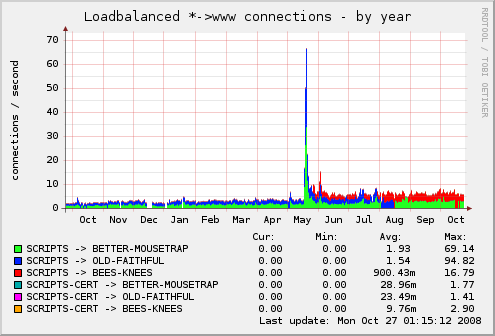
\includegraphics[width=3in] {Aggregated-cps_www-year.png}}
    \only<2>{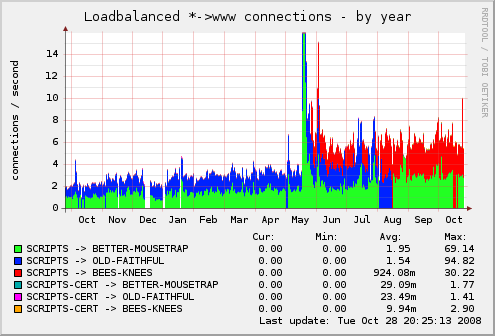
\includegraphics[width=3in] {Aggregated-cps_www-year-clip.png}}
  \end{center}
\end{frame}

\begin{frame}
  \frametitle{Load Balancing status}
  \begin{itemize}
  \item \url{http://scripts.mit.edu:78/} shows the current load
  \item Or you can \texttt{finger @scripts.mit.edu} for more detail
  \end{itemize}
\begin{verbatim}
  $ finger @scripts
[scripts.mit.edu]
IP Virtual Server version 1.2.1 (size=4096)
Prot LocalAddress:Port Scheduler Flags
  -> RemoteAddress:Port           Forward Weight ActiveConn InActConn
FWM  1 wrr
  -> CATS-WHISKERS.MIT.EDU:0      Route   1      13         6
FWM  2 wlc persistent 600
  -> SHINING-ARMOR.MIT.EDU:0      Route   4096   53         855
  -> BEES-KNEES.MIT.EDU:0         Route   4096   50         2140
  -> CATS-WHISKERS.MIT.EDU:0      Route   1024   17         53
  -> BUSY-BEAVER.MIT.EDU:0        Route   4096   54         641
  -> PANCAKE-BUNNY.MIT.EDU:0      Route   4096   52         1039
FWM  3 wlc persistent 600
  -> SHINING-ARMOR.MIT.EDU:25     Route   4096   0          0
  -> BEES-KNEES.MIT.EDU:25        Route   4096   0          1
  -> CATS-WHISKERS.MIT.EDU:25     Route   1024   0          1
  -> BUSY-BEAVER.MIT.EDU:25       Route   4096   0          1
  -> PANCAKE-BUNNY.MIT.EDU:25     Route   4096   0          2
\end{verbatim}
\end{frame}
